\documentclass{beamer}

\mode<presentation> {

%\usetheme{default}
%\usetheme{AnnArbor}
%\usetheme{Antibes}
%\usetheme{Bergen}
%\usetheme{Berkeley}
%\usetheme{Berlin}
%\usetheme{Boadilla}
%\usetheme{CambridgeUS}
%\usetheme{Copenhagen}
%\usetheme{Darmstadt}
%\usetheme{Dresden}
%\usetheme{Frankfurt}
%\usetheme{Goettingen}
%\usetheme{Hannover}
%\usetheme{Ilmenau}
%\usetheme{JuanLesPins}
%\usetheme{Luebeck}
\usetheme{Madrid}
%\usetheme{Malmoe}
%\usetheme{Marburg}
%\usetheme{Montpellier}
%\usetheme{PaloAlto}
%\usetheme{Pittsburgh}
%\usetheme{Rochester}
%\usetheme{Singapore}
%\usetheme{Szeged}
%\usetheme{Warsaw}


%\usecolortheme{albatross}
%\usecolortheme{beaver}
%\usecolortheme{beetle}
%\usecolortheme{crane}
%\usecolortheme{dolphin}
%\usecolortheme{dove}
%\usecolortheme{fly}
%\usecolortheme{lily}
%\usecolortheme{orchid}
%\usecolortheme{rose}
%\usecolortheme{seagull}
%\usecolortheme{seahorse}
%\usecolortheme{whale}
%\usecolortheme{wolverine}

%\setbeamertemplate{footline} % To remove the footer line in all slides uncomment this line
%\setbeamertemplate{footline}[page number] % To replace the footer line in all slides with a simple slide count uncomment this line

%\setbeamertemplate{navigation symbols}{} % To remove the navigation symbols from the bottom of all slides uncomment this line
}

\usepackage{graphicx} % Allows including images
\usepackage{booktabs} % Allows the use of \toprule, \midrule and \bottomrule in tables
\usepackage{amsfonts}
\usepackage{mathrsfs}
\usepackage{amsmath,amssymb,graphicx}

%----------------------------------------------------------------------------------------
%	TITLE PAGE
%----------------------------------------------------------------------------------------

\title["1.1"]{1.1: Examples of Time Series} 

\author{Taylor} 
\institute[UVA] 
{
University of Virginia \\
\medskip
\textit{} 
}
\date{} 

\begin{document}
%----------------------------------------------------------------------------------------

\begin{frame}
\titlepage 
\end{frame}
%----------------------------------------------------------------------------------------

\begin{frame}
\frametitle{Definitions}

\begin{block}{defn}
A {\bf time series} is a set of observations $x_t$, each one being recorded at a specific time $t$
\end{block}

\begin{block}{defn}
A {\bf discrete-time time series} is a time series in which the set $T_0$ of times at which observations are made is a discrete set.
\end{block}


\end{frame}

%----------------------------------------------------------------------------------------

\begin{frame}[fragile] %need fragile for verbatim env
\frametitle{Try Running the R Code!}

\begin{verbatim}
# 1.1
# Author: Taylor
# STAT 4170

# import data #
# change this depending on your computer
setwd("~/UVa/all_teaching/4170_data/")
wineData <- read.csv("wine.csv", header=F)
colnames(wineData) <- c("wine")

# plot #
plot(wineData$wine, col="blue",type="l", xlab = "time", 
                                ylab = "wine sales")
time <- 1:(nrow(wineData))
points(time, wineData$wine)

\end{verbatim}

\end{frame}

%----------------------------------------------------------------------------------------

\begin{frame}
\frametitle{Example}

\begin{center}
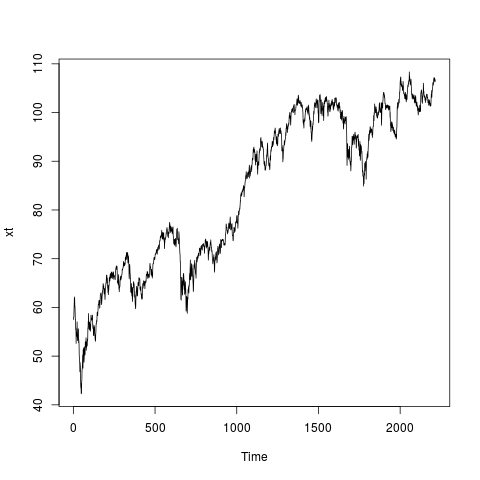
\includegraphics[width=100mm]{/home/taylor/UVa/all_teaching/4170_slides/1/1.1/pics/Rplot}
\end{center}

\end{frame}



\end{document} 